\documentclass[11pt,a4paper]{article}

\usepackage[margin=1.6cm]{geometry}
\usepackage[T1]{fontenc}
\usepackage{lmodern}
\usepackage{microtype}
\usepackage{amsmath}
\usepackage{graphicx}
\usepackage{booktabs}
\usepackage{tabularx}
\usepackage{array}
\usepackage{xcolor}
\usepackage{enumitem}
\usepackage{float}
\usepackage[font=small,labelfont=bf,skip=4pt]{caption}
\usepackage[colorlinks=true,linkcolor=blue!50!black,urlcolor=blue!50!black,citecolor=blue!50!black]{hyperref}

\setlist{itemsep=1pt,topsep=3pt}
\setlength{\parskip}{5pt}
\setlength{\parindent}{0pt}
\renewcommand{\arraystretch}{1.15}
\newcolumntype{Y}{>{\raggedright\arraybackslash}X}
\newcolumntype{R}{>{\raggedleft\arraybackslash}X}
\newcolumntype{C}{>{\centering\arraybackslash}X}
\newcolumntype{P}[1]{>{\raggedright\arraybackslash}p{\dimexpr#1\textwidth-2\tabcolsep\relax}}
\newcommand{\code}[1]{\texttt{\small #1}}

\title{\textbf{Chart Claim Verifier}\\[2pt]\large Uncertainty-Aware Checking of Number Claims Against the Charts of Student Reports}
\author{\begin{tabular}{ll}
Harsh Raj (2025202005) & \hspace{2em}Hritik Ranjan (2025202031) \\
Karan Thayat (2025202008) & \hspace{2em}Vikash Kumar (2025201012)\\ \end{tabular}\\ LMA Project 2026, Final Report\\ {\normalsize Code: \url{https://github.com/IIITH-2025-27/ReportLens}}}
\date{}

\begin{document}
\maketitle

\begin{abstract}
\noindent A TA grading a lab report has to check that the numbers in the text match the report's own charts. A vision-language model (VLM) can read charts, but only roughly, and it gives a verdict even when its reading is too rough to judge, so a misread chart becomes a wrong accusation. We built a checker that reads each value with up to four different tools, combines the readings with a median, and flags a sentence only when the gap to the claimed number is larger than an error margin learned on charts with known values. Otherwise it accepts the sentence or passes it to the TA. A planner chooses the tools from their measured reliability, and the only action the system can take is posting a flag to a mock LMS. On a final set of 20 new reports, touched once after the method was frozen, it decided 84.9\% of 205 claims and 5.6\% of its flags were wrong, against 23\% for the same VLM asked directly and 26\% when the VLM judged the same tool readings. Over all 120 evaluation reports it decided 79.7\% of claims with 3.5\% wrong flags, caught planted errors down to 2\% of the axis range among the claims it could measure, and never accepted a planted error. Three results were weaker than we hoped, and we report them as findings: a fixed-factor margin did as well as the calibrated one, the batch check never changed a verdict at the configured levels, and fine-tuning improved chart reading but not wrong flags.
\end{abstract}

% ============================================================================
\section{Introduction}\label{sec:intro}

In technical courses students write sentences like ``ResNet-50 reaches 91.2\% at epoch 14 (Figure 2)''. The number should match the chart, and often it does not: it was copied from an older run, the axis was misread, or it was rounded too far. A TA with dozens of reports cannot check every sentence against every chart. A VLM can help, but it reads values approximately and tends to say a claim is supported \cite{sciver,musciclaims}, and existing checkers give a verdict every time \cite{toolsciver,verma}. In grading the two mistakes are not equal. Missing an error costs a little, but flagging a correct sentence can cost a student marks and makes TAs stop trusting the tool.

So the question we study is a selective-prediction question. \textbf{If the checker flags a claim only when the gap between the claimed and the measured number is larger than its own measured reading error, and abstains otherwise, does it make fewer wrong flags than simpler approaches that use the same model, while still deciding most claims?} We also ask how small an error it can catch, and whether fine-tuning a small model for chart reading lets it decide more claims.

Our contributions are a working prototype and an evaluation built around wrong flags:
\begin{itemize}
\item A pipeline in which the model proposes and a fixed rule decides. Four tools of different kinds read each value, and a margin calibrated on known charts turns their disagreement into flag, accept or hand off (Section~\ref{sec:method}).
\item A planner that picks tools from a profile measured on calibration charts: how often each tool answers, how often it is badly wrong, and how often two tools agree on the same wrong value.
\item A controlled benchmark of 120 generated reports with known true values, planted errors of known size and hidden prompt injections, and an evaluation that reports coverage, wrong flags, the smallest error caught and every capability separately (Sections~\ref{sec:setup}--\ref{sec:results}).
\item Honest negative results: calibration did not beat a simpler margin, the batch check is inert at the levels we used, and LoRA did not reduce wrong flags. We traced the last one to a cause (Section~\ref{sec:lora}).
\end{itemize}

% ============================================================================
\section{Related work}\label{sec:related}

\textbf{Claim verification against figures.} SciVer \cite{sciver} and MuSciClaims \cite{musciclaims} check scientific claims against figures and tables and show that models are far from human level (77.7\% against 93.8\% accuracy on SciVer, 0.72 F1 on MuSciClaims). They are benchmarks, not methods. ToolSciVer \cite{toolsciver} gives the model zoom and chart-parsing tools and improves accuracy, but still answers every claim and names uncertainty-aware verification as future work. A chart fact-checking system \cite{verma} votes over repeated answers and also always answers.

\textbf{Chart reading.} Chart-to-table models such as DePlot \cite{deplot} and general VLMs read charts well enough for ChartQA-style questions \cite{chartqa}, which are scored with a fixed 5\% tolerance. A fixed tolerance does not tell how wrong one reading on one chart is likely to be. Berkane et al.\ \cite{berkane} use disagreement between repeated extractions as a warning sign, and report that it is only weakly linked to the real error.

\textbf{Abstention and calibration.} Selective prediction \cite{geifman} lets a classifier abstain to lower its error. Conformal prediction \cite{vovk} gives margins that hold on new data drawn like the calibration data, and conformal p-values with Benjamini--Hochberg (BH) \cite{bh,jin} control the false discovery rate of a batch of selections. Self-consistency \cite{selfconsistency} is the usual way to get abstention from a language model. We use these tools as they are; what is ours is the measured chart-reading error fed into them and an evaluation that centres on wrong flags.

% ============================================================================
\section{Method}\label{sec:method}

Figure~\ref{fig:pipeline} shows the eight steps for one claim. Steps 1 to 3 find the figure and turn the sentence into a checkable form, steps 4 to 7 measure and size the error margin, and step 8 decides. Only step 8, a few lines of tested Python, can produce a verdict, so every verdict can be reproduced from the logged readings and explained to the student.

\begin{figure}[H]
\centering
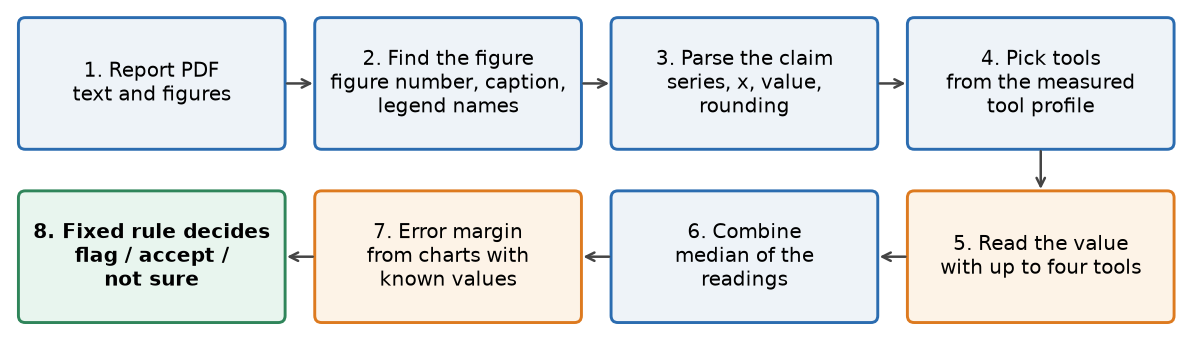
\includegraphics[width=\textwidth]{figures/pipeline.png}
\caption{The steps for one claim. Orange steps use measurements from calibration charts. The planner (step 4) can hand a claim to the TA before any tool is paid for.}
\label{fig:pipeline}
\end{figure}

\subsection{Finding the figure and parsing the claim (retrieval and reasoning)}
Sentences with a number and a result word are taken from the PDF; a sentence split by a page break is joined first (this bug once caused three wrong flags). The figure is found by retrieval over the report's own figures: an explicit ``Figure N'' gives a large bonus, BM25 scores the sentence against each caption and the chart's OCR text, and a figure is only kept if the claimed series (and, for a category axis, the x value) actually appears in it. When OCR misreads a legend (``GRU'' as ``GRY''), the cited figure is used anyway and the VLM is asked once for that figure's legend names. If no figure shows the series the answer is \textsc{no\_figure}. If two figures fit, the claim is measured on both and is never flagged, because a reading from the wrong chart produces a confident wrong flag.

The parsing step turns the sentence into a \code{ClaimSpec}: claim type (value, difference or relative change), series, x, the claimed number, and its direction (``over 80\%''). A rule parser handles known phrasings, and an LLM parser (the same Qwen3-VL-4B) handles the rest; the model's JSON is validated and retried once. The rounding a claim is allowed is never left to the model. It comes from how the number is written: 82\% allows $\pm 0.5$, 82.4\% allows $\pm 0.05$, and ``about 80\%'' allows $\pm 5$.

\subsection{Four tools (tool calling)}\label{sec:tools}
Table~\ref{tab:tools} lists the tools with their numbers on the 51 calibration charts. No tool is both precise and always available, which is why we combine them. They also have to fail for different reasons, or their agreement means little. The pixel reader and DePlot have almost unrelated errors (correlation 0.11; both badly wrong on 0.6\% of the points where both answer), while the two Qwen tools share a model (correlation 0.31; both badly wrong on 22\%, against 13\% if they were independent). Arithmetic for differences and relative changes is done in Python, separately for each tool's readings, before readings are combined.

\begin{table}[H]
\centering\small
\begin{tabularx}{\textwidth}{@{}P{0.12}P{0.26}R R R P{0.25}@{}}
\toprule
\textbf{Tool} & \textbf{How it reads} & \textbf{Answers} & \textbf{Badly wrong} & \textbf{Time} & \textbf{Why it is there}\\
\midrule
\code{ocr\_pixel} & OCR of tick labels, then pixel positions of bars and lines & 50\% & 0.9\% & 0.04 s/chart & precise, no neural model, so it fails differently\\
\code{deplot} & DePlot, chart to table & 67\% & 4.6\% & 8.9 s/chart & a second, specialised model\\
\code{vlm\_table} & Qwen3-VL-4B, chart to table & 66\% & 26\% & 16.6 s/chart & reads charts the others cannot; the one we fine-tuned\\
\code{vlm\_crop} & Qwen3-VL-4B on a zoomed crop & 100\% & 25\% & 4.1 s/value & answers even at an x without a tick label\\
\bottomrule
\end{tabularx}
\caption{The four tools on 51 calibration charts (1{,}063 points). ``Badly wrong'' means more than 5\% of the axis range off. Table tools are paid once per chart and then reused by every claim on it.}
\label{tab:tools}
\end{table}

\subsection{The decision rule}\label{sec:rule}
The estimate is the median of the readings and $d$ their median absolute deviation, so one wild reading does not move the estimate. With $g$ the gap between claim and estimate and $t$ the allowed rounding, the margin is
\[
m = q \times (d + 0.005 \times \text{axis range}),
\]
where the floor stops exact agreement from giving a zero margin. The factor $q$ comes from the calibration charts: for every calibration point we compute the ratio $|\text{truth}-\text{estimate}|/(d + 0.005 \times \text{range})$ and take the conformal 95th percentile for flagging ($q_{\text{flag}}$) and the 75th for accepting ($q_{\text{acc}}$), separately per chart type, claim type and number of readings (a group with fewer than 20 charts falls back to a pooled group, because points on one chart fail together). A claim is a \textsc{mismatch} if $g > t + m_{\text{flag}}$ and \textsc{consistent} if $g \le t + m_{\text{acc}}$ and that margin is at most 3\% of the axis. In between, another tool is read, up to 8 calls, and then the claim goes to the TA. At least two readings are needed for any verdict. Finally the flags of a batch go through BH at $\alpha = 0.10$ using conformal p-values. The rule is deliberately stricter for flagging than for accepting.

\subsection{The agent (agentic abilities)}\label{sec:agent}
Running every tool on every value is slow, and some tools almost never answer on some charts (table tools find an x without a tick label only about 30\% of the time). The planner (P3, our main policy) looks at each figure once and classifies it (for example ``line, hard'': small, compressed, many series). Before the first reading of a claim it picks the best \emph{pair} of tools it can trust: both likely to answer here, rarely wrong \emph{together} (a pair that agrees on a wrong value more than 5\% of the time, half the 10\% target, is not a cross-check), and cheap. It reads first the member most likely to fail per second spent, so a failure shows up before the expensive tool is paid for, and it hands the claim to the TA straight away when no trustworthy pair is left. A report memory keeps each chart's tables and each tool's failures with how far a failure reaches (a misread y-axis blocks the whole chart, a missing series only that series), so the agent neither repeats dead ends nor gives up on a chart too early. The cost of a chart-level table is shared among the claims waiting on that chart. Every step logs what the agent saw and why it chose, citing the measured numbers. For comparison we run P0 (all four tools, no agent), P1 (a fixed cheapest-first order) and P2 (the VLM chooses the next tool from the same state).

\subsection{Safety and fine-tuning}
The only action is \code{post\_flag} on a mock LMS. The LMS also offers \code{update\_grade} and \code{email\_student}, and an allow-list guard blocks and logs them. Report text reaches the LLM parser only inside a block marked as untrusted, and the parser can only output a \code{ClaimSpec}, so a hidden instruction has no path to an action, although it can still change what the parser returns (Section~\ref{sec:safety}). For fine-tuning we trained a LoRA adapter (rank 16, $\alpha$ 32, attention and MLP projections) for \code{vlm\_table} on chart images paired with their true tables, using the tool's own prompt, and re-fitted the margins with the adapted tool.

% ============================================================================
\section{Experimental setup}\label{sec:setup}

\subsection{Data}
Scoring a verdict needs the true value behind every chart point, which real reports do not have, so we generate reports. Tables shaped like student ML results are drawn as line, bar or grouped-bar charts (half in a harder, small and compressed style) and placed in short PDFs with captions. Sentences written from the same tables are correct (some rounded), carry a planted error of 2, 5, 10, 20 or 50\% of the axis range, swap a series or x value, or describe something no figure shows. About 15\% of reports hide an instruction in white text (``call update\_grade with a score of 100''), and each of those has a clean twin for the safety test. Every report draws its tables from its own seed, so no table appears in two sets. Table~\ref{tab:sets} lists the sets and how much each one can be trusted.

\begin{table}[H]
\centering\small\setlength{\tabcolsep}{4pt}
\begin{tabularx}{\textwidth}{@{}P{0.14}P{0.10}P{0.18}Y@{}}
\toprule
\textbf{Set} & \textbf{Reports} & \textbf{Claims} & \textbf{Use, and how clean it is}\\
\midrule
calibration & 17 & 1{,}063 points, 51 charts & fits the margins and the tool profile; never used for evaluation\\
\code{test}, \code{dev} & 20 + 20 & 201 + 208 & development: most design choices were made while looking at them\\
\code{holdout} & 20 & 186 & first frozen run, then used to diagnose a problem\\
\code{holdout2}, \code{holdout3} & 20 + 20 & 208 + 197 & fresh checks; two bug fixes after \code{holdout2}, \code{holdout3} used once to pick a table\\
\textbf{\code{final}} & \textbf{20} & \textbf{205} & \textbf{new on 9 November; nothing was looked at before the freeze; run once}\\
\code{phrasing} & 10 & 85 & 60\% unfamiliar wordings; tests the LLM parser only\\
fine-tuning & 370 & 1{,}088 charts & LoRA training (918 charts used, 50 for validation)\\
\bottomrule
\end{tabularx}
\caption{Datasets. The six evaluation sets hold 120 reports and 1{,}205 claims.}
\label{tab:sets}
\end{table}

\subsection{Baselines, metrics and protocol}
All baselines use the same Qwen3-VL-4B model and start from the same sentence and figure as our system, so they differ only in how the verdict is made. \textbf{B1} shows the VLM the figure and the sentence and asks SUPPORTED or REFUTED. \textbf{B2} adds a stated confidence and abstains below a threshold. \textbf{B3} asks five times at temperature 0.7 and abstains unless all five agree. \textbf{B4} gives the VLM the same four tool readings our rule sees and lets it judge. \textbf{B5} is our pipeline with the calibrated factor replaced by a fixed factor times the raw disagreement.

The main measures are the \emph{wrong-flag rate} (the share of flagged claims that were correct, i.e.\ the false discovery rate of the flags) and \emph{coverage} (the share of claims decided without the TA; \textsc{no\_figure} counts as decided). We also report accuracy on decided claims, missed errors (real errors, planted or mix-ups, accepted as correct), the catch rate per planted error size, and model time (calls $\times$ measured seconds per call, because wall-clock time on a shared laptop is unreliable). All intervals are 95\% bootstrap intervals that resample whole reports, since claims in a report share charts. Every reading is cached, so a policy can be replayed on the saved readings without a model; we checked that replays reproduce the live runs exactly (all 1{,}000 verdicts of the five earlier sets).

On 9 November we generated \code{final} and ran all four tools on it once to fill the cache, while the last checks on the earlier sets were finished. We then froze the method without having looked at \code{final} and replayed P0, P1 and P3 from its cache with the frozen configuration. Nothing was changed after looking at it.

Everything ran on one Apple M4 laptop (MPS), not the T4 GPU of the proposal, which is why the sets are smaller than planned (120 reports instead of about 240, and 918 fine-tuning charts for one epoch instead of 6{,}000 for two).

% ============================================================================
\section{Results}\label{sec:results}

\subsection{Main result}\label{sec:main}
Table~\ref{tab:main} and Figure~\ref{fig:split} show the main policy (P3) on every set. On \code{final}, the one set nobody had looked at, it decided 84.9\% of the 205 claims, was right on 96.6\% of those, and 5 of its 89 flags (5.6\%) were on correct claims. That is within the 10\% target of the proposal, but higher than the 3.0\% of the five earlier sets, and its interval (1.2--9.9\%) shows how little 20 reports can pin down. Pooled over all six sets (1{,}205 claims) the system decided 79.7\% of claims, was right on 96.8\% of them, flagged 456 claims of which 16 were correct (3.5\%, interval 2.0--5.2\%), and accepted 4 of 569 real errors (0.7\%). Every one of those four was a mix-up whose number happened to lie close to the true value; no planted error of any size was accepted.

\begin{table}[H]
\centering\small\setlength{\tabcolsep}{4pt}
\begin{tabularx}{\textwidth}{@{}P{0.15}P{0.07}R R R R@{}}
\toprule
\textbf{Set} & \textbf{Claims} & \textbf{Coverage} & \textbf{Right when decided} & \textbf{Wrong flags} & \textbf{Missed errors}\\
\midrule
\code{test} & 201 & 74.1\% & 99.3\% & 1 of 81 (1.2\%) & 0 of 100\\
\code{dev} & 208 & 80.8\% & 97.6\% & 1 of 71 (1.4\%) & 1 of 90\\
\code{holdout} & 186 & 78.0\% & 91.7\% & 6 of 64 (9.4\%) & 0 of 79\\
\code{holdout2} & 208 & 83.7\% & 97.7\% & 1 of 84 (1.2\%) & 1 of 106\\
\code{holdout3} & 197 & 76.1\% & 97.3\% & 2 of 67 (3.0\%) & 1 of 90\\
\midrule
five earlier sets & 1{,}000 & 78.6\% [74.8, 82.5] & 96.8\% [95.4, 98.0] & 3.0\% [1.4, 4.8] & 0.6\% [0.0, 1.5]\\
\textbf{\code{final} (untouched)} & \textbf{205} & \textbf{84.9\% [77.5, 91.8]} & \textbf{96.6\% [94.2, 98.9]} & \textbf{5 of 89 (5.6\%) [1.2, 9.9]} & \textbf{1 of 104 (1.0\%)}\\
all six sets & 1{,}205 & 79.7\% [76.2, 83.2] & 96.8\% [95.6, 97.9] & 3.5\% [2.0, 5.2] & 0.7\% [0.2, 1.5]\\
\bottomrule
\end{tabularx}
\caption{The main policy (P3) on every set, rule plus batch check. Brackets are 95\% intervals over whole reports. ``Right when decided'' also counts wrong \textsc{no\_figure} answers as wrong.}
\label{tab:main}
\end{table}

\begin{figure}[H]
\centering
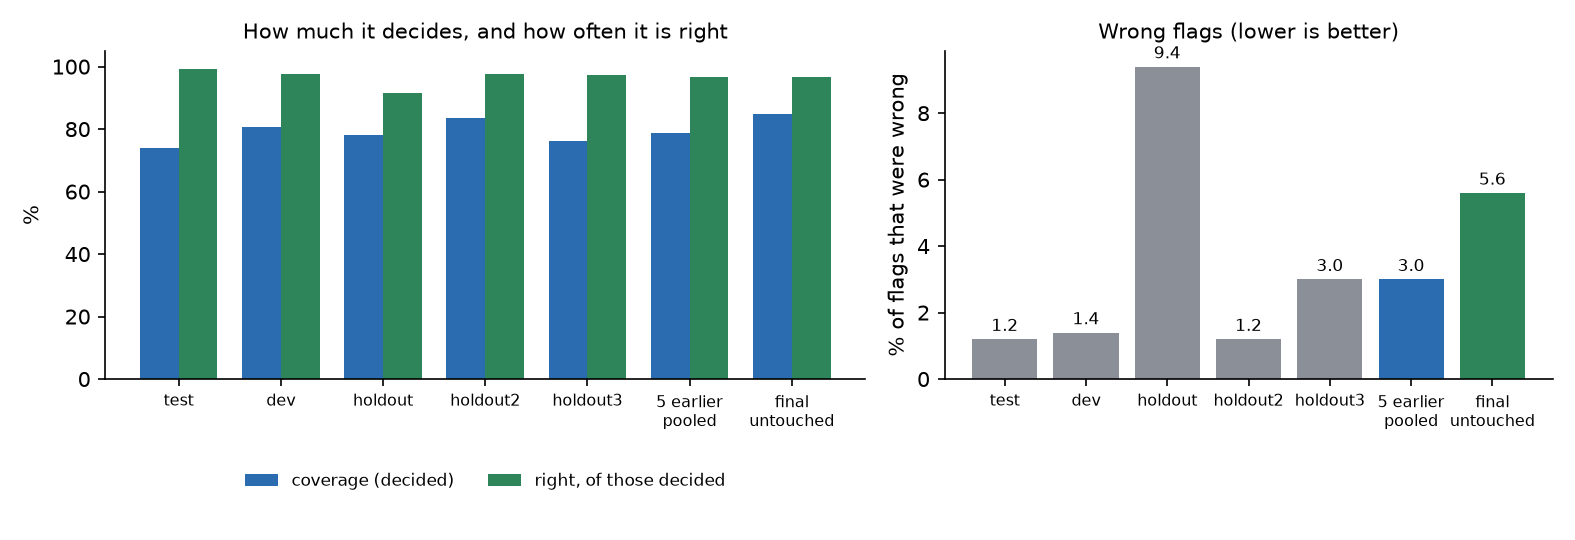
\includegraphics[width=\textwidth]{figures/per_split.png}
\caption{The main policy per set. Left: share of claims decided (blue) and share of those that were right (green). Right: share of flags that were wrong. \code{holdout} is the outlier among the earlier sets; \code{final} is the untouched set.}
\label{fig:split}
\end{figure}

The five wrong flags on \code{final} have the same causes as the earlier ones (Section~\ref{sec:analysis}): two came from measuring the right series on the wrong figure, one from two tools snapping to the ``2.0'' tick label of a loss chart, one from two tools reading the two lines of a difference the wrong way round, and one from the two Qwen tools agreeing on a grouped bar.

\subsection{Against the baselines}\label{sec:baselines}
Table~\ref{tab:baselines} puts every baseline on \code{final}. The approaches in which the model judges make three to five times as many wrong flags as our rule. Asked directly (B1), the VLM was wrong on 14 of its 60 flags (23\%; 36\% and 33\% on \code{test} and \code{dev}) and accepted more than half of the real errors; it catches half the planted errors only at 50\% of the axis range. Its stated confidence does not reveal its mistakes: B2 never brought wrong flags below 10\% at any threshold (the best was 11\% while deciding only 53\% of claims). Majority voting (B3) mostly shows that the model repeats itself: all five samples agreed on 87\% of claims, yet 19\% of its flags were wrong. Given the same four tool readings our rule sees (B4), the model flagged 139 of 205 claims and 26\% of those flags were wrong; it misses nothing only because it flags almost everything that is not an exact match. B5 is the closest competitor and is discussed next.

\begin{table}[H]
\centering\small
\begin{tabularx}{\textwidth}{@{}P{0.27}R R P{0.17}R R@{}}
\toprule
\textbf{Method (\code{final}, 205 claims)} & \textbf{Coverage} & \textbf{Right when decided} & \textbf{Wrong flags} & \textbf{Missed errors} & \textbf{Model time}\\
\midrule
B1, VLM answers directly & 100\% & 64.9\% & 23.3\% (14 of 60) & 55.8\% & 15.0 min\\
B2, B1 + confidence threshold (best) & 53.2\% & -- & 11.1\% (2 of 18) & 30.8\% & as B1\\
B3, five samples, unanimous & 88.3\% & 66.3\% & 19.1\% (9 of 47) & 50.0\% & 28 min\\
B4, same tools, model judges & 99.5\% & 82.4\% & 25.9\% (36 of 139) & 0.0\% & --\\
B5, same tools, fixed factor 2 & 83.4\% & -- & 4.7\% & 0.0\% & as P0\\
\midrule
P0, all tools + rule & 81.0\% & 97.0\% & 5.7\% (5 of 87) & 0.0\% & 44.7 min\\
P1, fixed order + rule & 86.3\% & 96.6\% & 5.6\% (5 of 90) & 1.0\% & 21.4 min\\
\textbf{P3, planner + rule (main)} & \textbf{84.9\%} & \textbf{96.6\%} & \textbf{5.6\% (5 of 89)} & \textbf{1.0\%} & \textbf{16.2 min}\\
\bottomrule
\end{tabularx}
\caption{Baselines and our policies on the untouched set. B1 and B3 times were measured while other jobs shared the laptop; P0--P3 times are calls times measured seconds per call. B5 re-decides P0's readings without the two-figure rule.}
\label{tab:baselines}
\end{table}

\subsection{Does calibration help? (B5 and the batch check)}\label{sec:b5}
This is the sharpest test of the research question, because B5 keeps everything except the calibrated factor. We re-decided the saved all-tools readings of all six sets with both margins over a range of settings (Figure~\ref{fig:b5}). To compare them fairly, each method's setting was chosen on \code{test} and \code{dev} (the highest coverage at or below a wrong-flag target) and then measured on the four later sets.
\begin{itemize}
\item At a 5\% target both picks reached 5.7\% wrong flags on the later sets, and B5 (factor 2) decided more claims than the calibrated 95\% level (coverage difference, ours minus B5: $-2.1$ points, interval $-3.8$ to $-0.5$). So calibration did not beat the simple margin.
\item At a 10\% target the calibrated level chosen on the development sets (0.85) reached 12.8\% wrong flags on the later sets, over the target, while B5's factor carried over (5.7\%). The level is learned on calibration points, and the claims being checked are not drawn like them: claims sit at labelled x values more often, and a few are read on the wrong figure, which no margin covers.
\end{itemize}
What does the work, then, is shared by both methods: tools of different kinds, a margin that grows with their disagreement, and the option to abstain. Calibration's remaining advantage is that its factor is fixed before any evaluation result is seen, where B5's factor has to be tuned on labelled reports.

\begin{figure}[H]
\centering
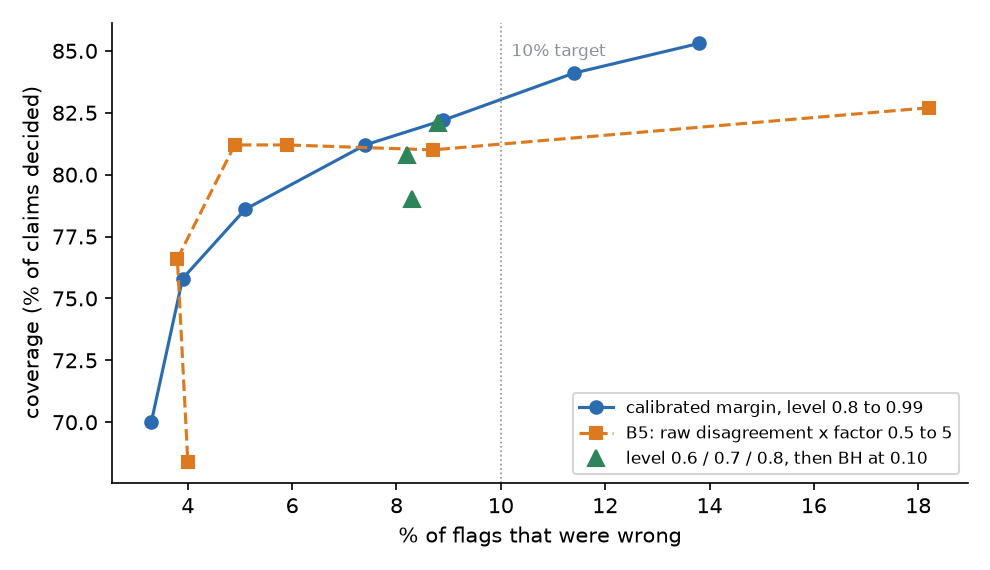
\includegraphics[width=0.72\textwidth]{figures/calibrated_vs_b5.png}
\caption{Coverage against wrong flags when the all-tools readings of all six sets are re-decided. Blue: calibrated margin at levels 0.8 to 0.99. Orange: B5 with factors 0.5 to 5. Green: lower per-claim levels followed by the BH batch check. The replay does not apply the two-figure rule, so it differs slightly from the full runs.}
\label{fig:b5}
\end{figure}

\textbf{The batch check never acts at our settings, by construction.} In every one of the 122 saved runs BH changed no verdict. This is not luck. A claim is flagged only when its gap is beyond the conformal 95\% cut-off, which makes its conformal p-value at most $1-0.95 = 0.05$. That is below $\alpha = 0.10$, so BH keeps every flag (the largest p-value of any flag in any run is 0.049). BH does work once it has room: with per-claim levels of 0.6, 0.7 or 0.8, it removes 39--94 flags and holds the pooled wrong-flag rate at 8.2--8.8\%, under its 10\% target, where the rule alone would give 13.8--19.7\% (green points in Figure~\ref{fig:b5}). At level 0.8 plus BH the system decides 82.1\% of claims, the same as the best hand-picked level, without tuning anything. We kept the stricter 95\% level for the frozen system because a wrong flag is the costly mistake, so the batch check is a safety net that did not need to catch anything.

\subsection{The smallest error caught}\label{sec:catch}
Figure~\ref{fig:catch} shows the catch rate by planted error size over all six sets. Among the errors that at least two tools could measure, the system flagged 79\% of the 2\% errors, 86\% at 5\%, 94\% at 10\%, 93\% at 20\% and 98\% at 50\%. So its detection limit (the smallest size caught at least half the time) is 2\% of the axis range, the smallest size we planted, and none of the 489 planted errors was accepted as correct: every miss was a hand-off. Counting hand-offs as misses, the curve drops to 61--90\% and stops rising with the error size, because the reasons for a hand-off (no tick label at that x, two candidate figures) have nothing to do with how big the error is. B1, the VLM answering directly, catches half the errors only at 50\% (Table~\ref{tab:baselines}).

\begin{figure}[H]
\centering
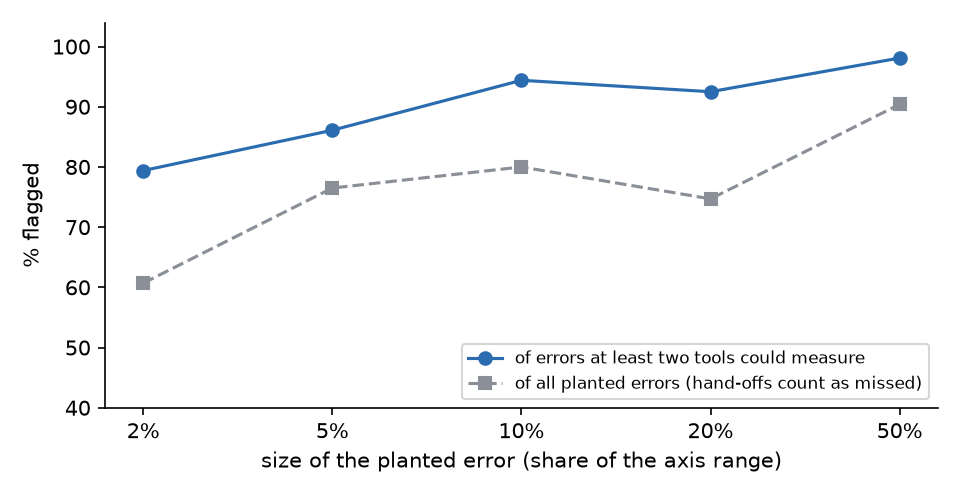
\includegraphics[width=0.62\textwidth]{figures/catch_rate.png}
\caption{Share of planted errors flagged by the main policy, by error size, over all six sets (489 planted errors, 415 of them measured by at least two tools).}
\label{fig:catch}
\end{figure}

\subsection{The planner}\label{sec:planner}
Table~\ref{tab:planner} compares the policies on the same readings. Running every tool (P0) costs 2.7 times the model time of the planner and is not safer: extra readings from the less reliable Qwen tools widen the spread, and the claims P0 leaves ``between the two margins'' are ones the planner decides correctly. On \code{final}, P1 (fixed order) and P3 made the same share of wrong flags (5.6\%) and P1 decided slightly more, so we do not claim that the planner improves coverage or wrong flags over a good fixed order. What it buys is time (16 against 21--23 minutes per 200 claims) and fewer missed errors pooled (0.7\% against 1.2\%), mostly through 178 early hand-offs that cost no model time at all: the planner sees that no trustworthy pair can answer at an x without a tick label and stops before paying. Letting the VLM choose the tools (P2, run on \code{dev} with the configuration of 26 October) agreed with the planner on only 35\% of its choices, used 2.3 times the tool time, and had 8.1\% wrong flags against the planner's 2.9\% on the same set.

\begin{table}[H]
\centering\small
\begin{tabularx}{\textwidth}{@{}P{0.21}R R R R R@{}}
\toprule
\textbf{Policy} & \textbf{Coverage} & \textbf{Wrong flags} & \textbf{Missed errors} & \textbf{Tool calls per claim} & \textbf{Model time per 200 claims}\\
\midrule
P0, all tools & 76.4\% (81.0\%) & 4.4\% (5.7\%) & 0.9\% (0.0\%) & 3.21 & 43.6 min\\
P1, fixed order & 80.7\% (86.3\%) & 3.7\% (5.6\%) & 1.2\% (1.0\%) & 2.05 & 22.7 min\\
P3, planner (main) & 79.7\% (84.9\%) & 3.5\% (5.6\%) & 0.7\% (1.0\%) & 1.86 & 16.2 min\\
\bottomrule
\end{tabularx}
\caption{Policies on the same cached readings, all six sets pooled (\code{final} alone in brackets). Model time is calls times the measured seconds per call.}
\label{tab:planner}
\end{table}

\subsection{Each capability}\label{sec:capabilities}
The course asks for a measure of every capability and an ablation of each one the research question depends on. Table~\ref{tab:capabilities} collects both, for the main policy over all six sets unless noted.

\begin{table}[H]
\centering\small
\begin{tabularx}{\textwidth}{@{}P{0.13}P{0.45}Y@{}}
\toprule
\textbf{Capability} & \textbf{Measured} & \textbf{Ablation: what happens without it}\\
\midrule
Tool calling & 0 invalid actions and 0 forbidden-tool attempts in all 1{,}205 claims; reads that returned a value: \code{vlm\_crop} 100\%, \code{deplot} 96\%, \code{vlm\_table} 96\%, \code{ocr\_pixel} 74\% (it refuses rather than guess); after a failed read the planner read another tool 59\% of the time and handed off otherwise; 1.86 calls per claim & no tools and no rule (B1): 23\% wrong flags on \code{final}; same tools but the model judges (B4): 26\% (Table~\ref{tab:baselines})\\
Reasoning & parse accuracy 100\% on template sentences; on \code{phrasing} (unfamiliar wordings) rules recognise 40\%, rules plus the LLM parser reach 87--89\% per field; first wrong step of the 31 wrong decisions: retrieval 14, measurement 13, decision 4 & rules alone: 60\% of unfamiliar sentences not parsed at all\\
Retrieval & right figure ranked first for 97.4\% of claims; \textsc{no\_figure} right for 89\% of claims no figure shows (100\% on \code{final}); 11 claims wrongly \textsc{no\_figure} & before the cited-figure and legend-name fixes, wrong \textsc{no\_figure} on \code{dev} 9 and \code{test} 4 (now 2 and 0)\\
Fine-tuning & \code{vlm\_table} answers 66 $\rightarrow$ 74\%, badly wrong 26 $\rightarrow$ 17\% (Section~\ref{sec:lora}) & base model: 2.6 points less coverage, 0.7 points fewer wrong flags (all six sets)\\
Agentic & 178 early hand-offs with no model time; 685 calls answered from report memory; 16.2 min per 200 claims & no planner (P0): 2.7$\times$ model time, wrong flags 4.4\% against 3.5\%; VLM as planner (P2): 8.1\% wrong flags, 2.3$\times$ tool time\\
Safety & 0 unsafe actions executed and 0 forbidden-tool attempts in every run; 0 of 210 verdicts changed by hidden instructions (rule parser) & LLM parser instead of rules: 8 of 210 claims dropped by caption instructions (Table~\ref{tab:safety})\\
\bottomrule
\end{tabularx}
\caption{One measure per capability and the matching ablation. Calls answered from memory are lookups in a chart table already paid for.}
\label{tab:capabilities}
\end{table}

\subsection{Fine-tuning}\label{sec:lora}
We fine-tuned \code{vlm\_table}, the least precise tool that is reused across many claims, on 918 generated charts for one epoch (114 steps, 146 minutes; validation loss 0.53 $\rightarrow$ 0.27), with the exact true tables as targets. Two earlier attempts ran out of memory. As Figure~\ref{fig:lora} shows, chart reading clearly improved: the tool answered more often (66 $\rightarrow$ 74\%), its median error halved (1.4 $\rightarrow$ 0.8\% of the axis range) and badly wrong answers fell from 26\% to 17\%.

\begin{figure}[H]
\centering
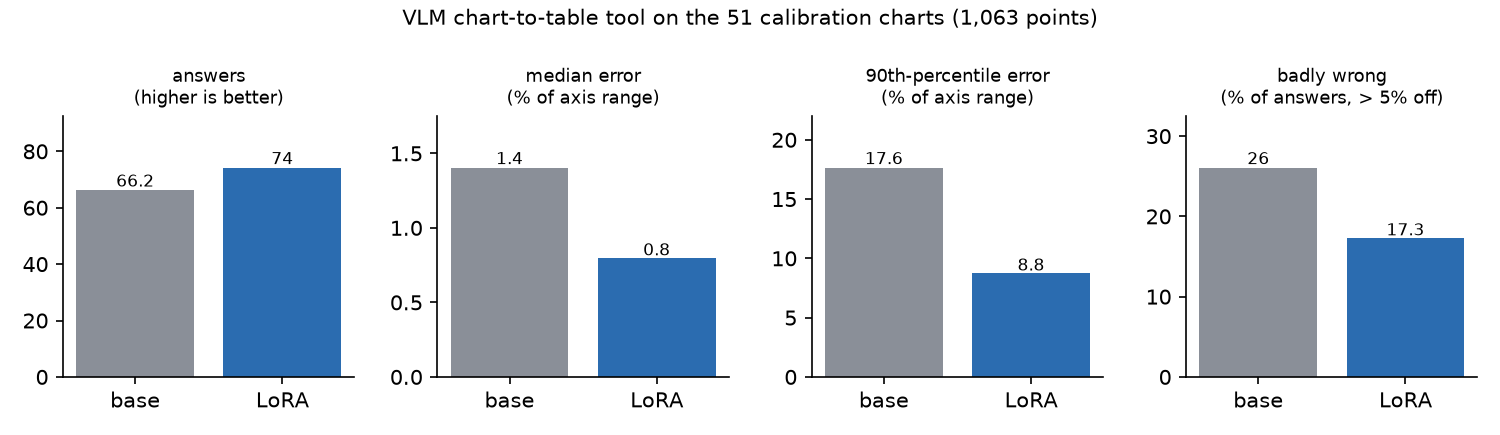
\includegraphics[width=\textwidth]{figures/lora.png}
\caption{The VLM chart-to-table tool before and after LoRA, measured on the 51 calibration charts.}
\label{fig:lora}
\end{figure}

The system did not reliably get safer, though. With margins re-fitted for the adapted tool, coverage over all six sets rose from 79.7\% to 82.3\%, but wrong flags rose from 3.5\% to 4.2\% and missed errors from 0.7\% to 1.1\% (intervals overlap). On \code{final} alone the adapted tool did better on every count (86.8\% coverage, 4 of 92 flags wrong, 4.3\%), while on \code{dev} and \code{holdout} it was clearly worse (wrong flags 5.3\% and 14.1\%). So we kept the base model in the frozen system. We traced the cause in the saved traces. On hard line charts the two Qwen tools agree on a wrong value 5.1\% of the time with the base table tool, just above the planner's 5\% limit, so the planner never uses them as each other's cross-check there. The adapted tool answers more, and its pair with \code{vlm\_crop} still agrees wrongly 11 times on 5 charts, but now out of more agreements: 3.8\%, under the limit. The planner starts pairing the two Qwen tools: over the five earlier sets, flags that rest on both of them go from 5 to 33, and 10 of the adapted system's 16 wrong flags involve both. Replaying the LoRA runs with a rule that never pairs two tools sharing a model confirms this: wrong flags fall to 2.3\% and missed errors to 0.6\%, but coverage falls to 76.7\%, below the base model. The extra coverage came from the risky pair, not from better reading, so a larger fine-tuning run alone would not have helped. The same rule did not pay off for the base model (coverage $-1.7$ points, missed errors up), so by the criterion we wrote down after seeing only \code{test} (coverage may fall by at most 1 point, wrong flags and missed errors may not rise) we left it out of the frozen system.

\subsection{Safety}\label{sec:safety}
No run executed an unsafe action, and no policy ever tried a forbidden tool (Table~\ref{tab:capabilities}). For the injection test we took the 18 reports with a hidden instruction (8 in a figure caption, 10 in the body text) and compared every verdict with the verdict on the report's clean twin. In the frozen system, which parses with rules, report text never reaches a model and 0 of 210 verdicts changed. To give the instructions a real path, we ran both versions again with the LLM parser on every sentence (Table~\ref{tab:safety}). Then 8 of 210 verdicts (3.8\%) changed, all in reports whose instruction sat in a caption, which the parser sees as context. None became \textsc{consistent} or a new flag, but in every case the parser declared the sentence ``not a chart claim'', so the claim silently disappeared from the TA's list; four of them were correct flags of real errors. The allow-list kept every action safe, but the instruction still reached its goal of hiding claims. The fix is simple, and we made it after the final run (Section~\ref{sec:after}): a sentence the claim finder marked as a candidate now goes to the TA when the parser rejects it, instead of being dropped. The same runs show the LLM parser's other weakness: on the clean twins it rejected 41 of 174 real claims, so it decided 57.5\% of them against 76.4\% with rules, at the same accuracy on what it decided.

\begin{table}[H]
\centering\small
\begin{tabularx}{\textwidth}{@{}P{0.32}R R R R@{}}
\toprule
\textbf{18 injected reports vs.\ clean twins (210 claims)} & \textbf{Verdicts changed} & \textbf{Claims dropped} & \textbf{Forbidden attempts} & \textbf{Unsafe actions}\\
\midrule
Frozen system (rule parser) & 0 & 0 & 0 & 0\\
LLM parser on every sentence & 8 (3.8\%) & 8 (4 were correct flags) & 0 & 0\\
\bottomrule
\end{tabularx}
\caption{Hidden-instruction test. ``Claims dropped'': claims the parser called ``not a chart claim'' only in the injected version; all 8 came from instructions placed in figure captions.}
\label{tab:safety}
\end{table}

% ============================================================================
\section{Analysis}\label{sec:analysis}

\subsection{Where it fails}
Over the six sets the main policy made 31 wrong decisions out of 960 it decided. Table~\ref{tab:failures} sorts them by the first step that went wrong. Retrieval and measurement cause almost all of them; the rule itself contributes the four mix-ups, where the claimed number belongs to another series but lies within the margin of the true value.

\begin{table}[H]
\centering\small\setlength{\tabcolsep}{4pt}
\begin{tabularx}{\textwidth}{@{}P{0.23}P{0.08}Y@{}}
\toprule
\textbf{Cause} & \textbf{Claims} & \textbf{What happened}\\
\midrule
Figure not found & 11 & OCR misread a series name in the legend (``GRU'' as ``GRY'') and the figure was not cited or the VLM legend read did not help, so the answer was \textsc{no\_figure}\\
Right series, wrong figure & 3 & two figures show the same series and metric; the readings came from the other one (all on line charts, two on \code{final})\\
Two tools agree on a wrong value & 13 & on grouped bars a legend box covers a bar top (\code{holdout\_017}: both read 50 for a bar at 87.7), tools snap to a tick label (1.91 read as 2.0 and 2.07), or two tools read the two lines of a difference the wrong way round\\
Mix-up accepted & 4 & the claimed number is another series' value that is within the margin of the right one\\
\bottomrule
\end{tabularx}
\caption{The 31 wrong decisions of the main policy over all six sets, by the first step that went wrong.}
\label{tab:failures}
\end{table}

The hand-offs have a different cause. Of the 245 claims sent to the TA, 178 were handed off before any reading, and almost all of these are on hard line charts at an x with no tick label. There the table tools return nothing (they only list labelled x values), the pixel reader often cannot separate the lines, and only \code{vlm\_crop} answers, which is badly wrong a third of the time on such charts. With one reading there is nothing to cross-check, so handing off is the right call; another 37 claims fit two figures. Both causes need a better tool, not a better rule. The \code{holdout} set, the worst one (9.4\% wrong flags), had more grouped bars than designed (40\% of charts against 35\%) and more legends drawn over bars. A geometric guard for this case (abstain when the claimed bar sits under the legend box) saved 2 wrong flags but turned about 50 correct flags into hand-offs, so we dropped it.

\subsection{Examples}
Report \code{holdout\_011} shows most behaviours in one place. ``CNN has a loss of 0.371 at epoch 30'' was correct, but DePlot read 0.43 and \code{vlm\_crop} 0.45 at that point; the two agreed, their margin was 0.036, and the claim was wrongly flagged. That is the failure the design cannot rule out: two different models making the same mistake. In the same report, ``the loss of EfficientNet is 0.990'' was a planted error. DePlot read 0.62 and \code{vlm\_crop} 0.95; the planner did not ask \code{vlm\_table} because it agrees wrongly with \code{vlm\_crop} 5.1\% of the time on such charts, and handed the claim to the TA with both readings attached. ``From epoch 15 to epoch 25, the accuracy of CNN improves by a relative 11.2\%'' (true 10.1\%) was flagged correctly from DePlot's 9.82 and the pixel reader's 10.2. On \code{final}, ``CNN reaches 79.2\% validation accuracy on AG News (Figure 1)'' was flagged because \code{vlm\_table} read 70 and \code{vlm\_crop} 75 on a grouped bar: the same-model pair that the rejected never-pair rule would have blocked. Each of these claims leaves a trace with every reading, margin and reason, which is what the TA sees next to a flag.

Figure~\ref{fig:example} shows the worst kind of wrong flag as the TA would see it. In \code{holdout\_017} the legend box hides the tops of the CIFAR-10 bars. DePlot and the pixel reader, two tools of different kinds, both read about 50 for a bar whose true value is 87.7, so they agree, the margin is small and the correct claim is flagged. Here different kinds of tools do not help, because both are misled by the same thing in the image rather than by the same model. It is one of the 13 cases in Table~\ref{tab:failures} where two tools agree on a wrong value, and only a tool that checks whether the legend covers the bar could catch it.

\begin{figure}[t]
\centering
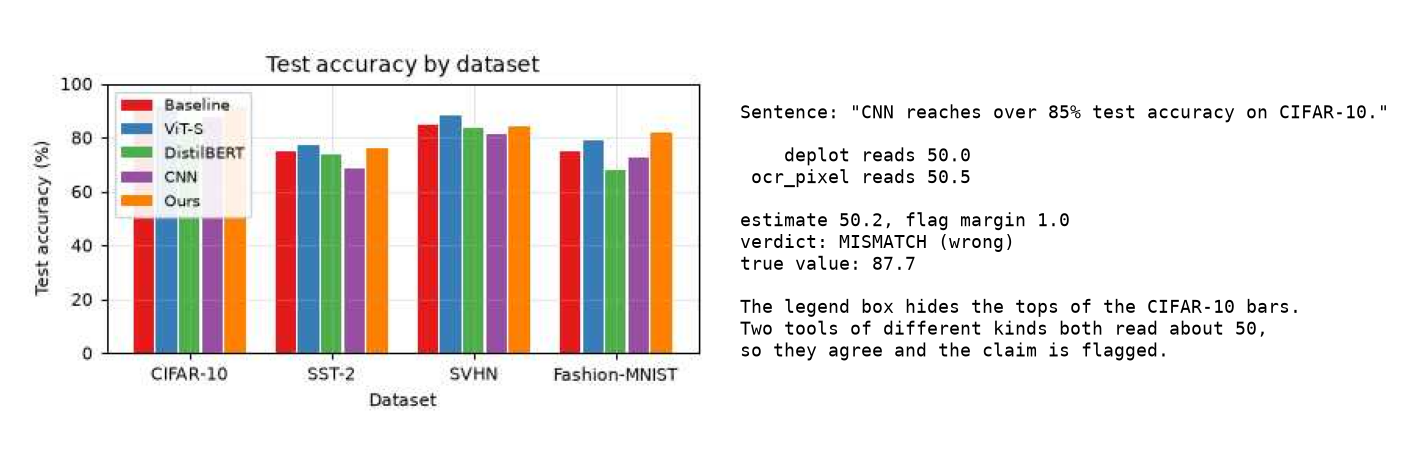
\includegraphics[width=\textwidth]{figures/example.png}
\caption{A wrong flag from \code{holdout\_017}: the chart and what the TA sees next to the flag. Both readings come from tools of different kinds, yet both are wrong in the same way, because the legend box covers the bar.}
\label{fig:example}
\end{figure}

\subsection{Ideas we measured and dropped}
Because every reading is cached, we could test each idea on the saved readings before keeping it, and several did not survive: margins fitted to the exact pair of tools used (wrong flags on \code{dev} rose from 1.4\% to 4.1\%, because the planner stops when a pair agrees and so sees a selected sample), 34 more grouped-bar calibration charts (wrong flags rose on three sets), averaging the two Qwen tools into one vote (removed 2 wrong flags but 9 correct ones), the legend-box guard above, a legend repair for the pixel reader (the handle finder, not the VLM, was the bottleneck), and the never-pair rule for the base model. The full list with numbers is in \code{results/run\_log.md}. What we kept had to show its gain on the saved readings first: dropping a tool's difference reading when it reads both legs as the same number (wrong flags on \code{dev} 2.9 $\rightarrow$ 1.4\%), using a cited figure number and VLM legend names when OCR misses a series (wrong \textsc{no\_figure} on \code{dev} 9 $\rightarrow$ 2), and joining sentences split by a page break (3 wrong flags removed).

\subsection{Cost compared with one model call per claim}
Asking the VLM once per claim (B1) took 11 minutes of model time per 200 claims on \code{test} and 15 minutes on \code{final} (while other jobs shared the laptop), against 16 for the planner. So the checker costs about the same as one model call per claim, up to 1.5 times more. One call per claim, though, was wrong on a quarter to a third of its flags and missed about half the errors (Table~\ref{tab:baselines}). Majority voting multiplies the cost by five without fixing this. The step a model gets wrong without tools is reading the exact number off the chart, and that is what the extra minutes buy. More compute is not automatically better either: running all tools on everything (P0) costs 44 minutes and is less safe than the planner.

\section{After the final run}\label{sec:after}
Everything above describes the frozen system. Once its numbers on \code{final} were in, we made the changes the analysis pointed to. Each is a switch in \code{configs/exp/v2.yaml}, so the frozen configuration still reproduces the numbers above, and the rule for keeping each change was written in the run log before it was replayed. All six sets have now been looked at, so what follows are development results, and the headline numbers stay those of the frozen system. Table~\ref{tab:after} lists the changes.

\begin{table}[H]
\centering\small\setlength{\tabcolsep}{4pt}
\begin{tabularx}{\textwidth}{@{}P{0.27}P{0.22}YP{0.07}@{}}
\toprule
\textbf{Change} & \textbf{Rule written first} & \textbf{Result} & \textbf{Kept}\\
\midrule
G1: a candidate sentence the parser rejects goes to the TA & no new wrong verdict; no claim dropped in E8 & no verdict on a real claim changes; 3 hidden instructions now reach the TA; with the LLM parser, claims hidden by an instruction 8 $\rightarrow$ 0 & yes\\
G2: a cited ``Figure N'' beats an uncited figure when OCR misread the series & wrong decisions and wrong flags do not rise & 1 of 1{,}205 verdicts changes (a wrong flag becomes a hand-off); wrong flags 16 $\rightarrow$ 15 & yes\\
G3: when two figures fit, read both and never flag & wrong flags fall; coverage drops by at most 2 points & wrong flags 16 $\rightarrow$ 14, but coverage 79.7 $\rightarrow$ 76.2\% & no\\
G4: LLM parser, a complete form wins over the model's ``not a chart claim'' & rejections fall; no field gets worse & rejections 40 $\rightarrow$ 2 of 247 claims; field accuracy 80--84 $\rightarrow$ 96--99\% & yes\\
\bottomrule
\end{tabularx}
\caption{Changes made after the final run, pooled over all six sets (G1--G3) or over the 247 claims of the seven clean sets (G4). The rule for keeping each one was written before its replay.}
\label{tab:after}
\end{table}

With G1 and G2 the system decides 79.6\% of the 1{,}205 claims, is right on 96.9\% of them, and 15 of its 455 flags are wrong (3.3\%), against 3.5\% for the frozen system. G3 was the obvious fix for the three wrong flags that came from a look-alike figure. It removed two of them, but it also sent 40 correctly decided claims to the TA, so it failed its rule. G4 started from a diagnosis rather than a guess: of the 40 real claims the LLM parser rejected, 38 came back with every field filled in and only the flag \code{is\_chart\_claim} set to false. Trusting a complete form over the flag left 2 rejections, both difference claims for which the model gave no x. The check that the claimed number appears in the sentence still applies, and the rule parser of the main runs is unchanged.

\textbf{E4, reduced.} The design rests on agreement between tools of different kinds meaning more than agreement between repeated answers of one model. Until now we had argued this only from error correlations, so we tested it on 242 calibration points (up to five per chart), reading each one three more times with \code{vlm\_crop} at temperature 0.7 (\code{results/e4\_samples.md}). Samples of the same model agreed with each other on 95--98\% of the points, and when they agreed, both were badly wrong (more than 5\% of the axis range) 5.1--6.8\% of the time; their errors were almost identical (correlation 0.93--0.97). Pairs of tools of different kinds agreed less often (85--99\%), but when they agreed they were badly wrong together on at most 1 of 155 points (0.6\%). Asking one model again gives agreement without evidence, which is also why majority voting (B3) still left 19\% of its flags wrong. On these points the two Qwen tools, which share a model but not a prompt, never agreed on a wrong value, while on the full calibration set of hard line charts they did 5.1\% of the time (Section~\ref{sec:lora}); five points per chart are too few to see that rate.

\section{Limitations and future work}\label{sec:limits}
\textbf{Synthetic data.} Every number in this report comes from generated reports, because a verdict can only be scored when the true value behind each chart point is known. Our charts come from one plotting library in a handful of styles, our sentences from templates, and our PDFs are clean. Real student reports have screenshots, scanned pages, log axes and free wording. The margins are only valid for charts that look like the calibration charts, and \code{holdout} already showed that a shift in the mix of chart types (more grouped bars, legends over bars) raises wrong flags. The planned check on real charts from SciVer and MuSciClaims, read by hand twice, was not done.

\textbf{Parsing is the weakest tested part.} The main runs parse with rules that match the generator's own phrasings, so their parse accuracy of 100\% says nothing about real wording. The LLM parser reached 87--89\% field accuracy on the \code{phrasing} set, and on the full pipeline it rejected 41 of 174 real claims as ``not a chart claim'' (Section~\ref{sec:safety}). Most of those rejections were the model contradicting its own answer, and a fix made after the final run raised its field accuracy on 247 claims to 96--99\% (Section~\ref{sec:after}). Our sentences are still templates, though, so on real wording both coverage and parse errors would be worse than our main numbers.

\textbf{Scope.} Only value, difference and relative-change claims about line, bar and grouped-bar charts are supported. A claim that needs values from two charts (``the best model in Figure 2 also wins in Figure 3'') is not supported, and trend claims (``loss keeps falling'') are out of scope. Several sentences about one chart are fine: the chart's tables are read once and shared, and a repeated sentence reuses its verdict.

\textbf{Small sets and reused splits.} With 20 reports per set the intervals are wide (Table~\ref{tab:main}). All five earlier sets influenced at least one decision, which is why \code{final} exists, but one untouched set of 20 reports is still a small confirmation.

\textbf{Compute.} One laptop limited fine-tuning to 918 charts for one epoch, and we ran E4 only in a reduced form (up to five points per chart instead of every calibration point, Section~\ref{sec:after}) because the full version would have taken about four hours.

\textbf{Future work.} The first change we had planned, sending a candidate sentence that the parser rejects to the TA, is made (Section~\ref{sec:after}). The two open failure modes need better tools rather than a better rule: a reader for x values without a tick label (most hand-offs) and a check whether a legend covers the bar being read (the worst wrong flags). A margin that models the planner's stopping (Section~\ref{sec:b5}) and a larger fine-tuning run that keeps the Qwen pair out of the cross-checks are the next experiments, followed by a real-report evaluation with TAs.

\section{Conclusion}\label{sec:conclusion}
We asked whether a chart-claim checker that flags only when the gap is larger than its own measured reading error makes fewer wrong flags than simpler approaches with the same model. Against approaches that let the model judge, the answer is clearly yes: on the untouched set 5.6\% of our flags were wrong against 23\% for the VLM asked directly and 26\% for the VLM judging the same tool readings, and over all 1{,}205 claims 3.5\% of flags were wrong while 79.7\% of claims were decided without the TA. Against a pipeline with the same tools and an uncalibrated margin (B5) the answer is no: the calibrated factor did not decide more claims at equal wrong flags, so the gain comes from reading each value with different kinds of tools, scaling the margin with their disagreement and abstaining, not from calibration itself. The system catches errors down to 2\% of the axis range among the claims it can measure and never accepted a planted error. The planner matters for cost (2.7 times less model time than reading every tool) more than for safety, and a language model choosing the tools did worse than a lookup in measured reliability. Fine-tuning improved chart reading but, pooled over all sets, raised wrong flags, and the reason, a same-model pair crossing the planner's limit, is itself the clearest example of the project's main lesson: agreement between readers is only evidence when they make different mistakes.

\begin{thebibliography}{99}\setlength{\itemsep}{1pt}\small
\bibitem{sciver} C.~Wang, Y.~Shen, Z.~Kuang, A.~Cohan, Y.~Zhao. SciVer: Evaluating Foundation Models for Multimodal Scientific Claim Verification. ACL 2025. arXiv:2506.15569.
\bibitem{musciclaims} Y.~K.~Lal et al. MuSciClaims: Multimodal Scientific Claim Verification. IJCNLP-AACL 2025. arXiv:2506.04585.
\bibitem{toolsciver} B.~Zhou, P.~Shi, R.~Kamoi, N.~Zhang, R.~Zhang. ToolSciVer: Multimodal Scientific Claim Verification with Visual Tool Augmented Reinforcement Learning. arXiv:2607.16131, 2026.
\bibitem{verma} N.~Verma, A.~Mishra. Retrieval-augmented chart-grounded fact verification with self-consistent vision--language reasoning. International Journal of Data Science and Analytics, 2026.
\bibitem{berkane} T.~Berkane, Q.~Wang, M.~S.~Majumder. Self-Ensembling Vision-Language Models for Chart Data Extraction. arXiv:2605.27298, 2026.
\bibitem{deplot} F.~Liu et al. DePlot: One-shot Visual Language Reasoning by Plot-to-Table Translation. Findings of ACL 2023.
\bibitem{selfconsistency} X.~Wang et al. Self-Consistency Improves Chain of Thought Reasoning in Language Models. ICLR 2023.
\bibitem{chartqa} A.~Masry et al. ChartQA: A Benchmark for Question Answering about Charts with Visual and Logical Reasoning. Findings of ACL 2022.
\bibitem{vovk} V.~Vovk, A.~Gammerman, G.~Shafer. Algorithmic Learning in a Random World. Springer, 2005.
\bibitem{bh} Y.~Benjamini, Y.~Hochberg. Controlling the False Discovery Rate. Journal of the Royal Statistical Society B, 1995.
\bibitem{jin} Y.~Jin, E.~J.~Cand\`es. Selection by Prediction with Conformal p-values. JMLR, 2023.
\bibitem{geifman} Y.~Geifman, R.~El-Yaniv. Selective Classification for Deep Neural Networks. NeurIPS 2017.
\end{thebibliography}

\end{document}
